\section{Dise�o detallado de m�dulos}

Los componentes que forman la aplicaci�n son el componente de la GUI, el de los Controlladores, el componente de Epanet y el componente Metaheuristico. La relaci�n entre los componentes puede ser apreciada en la Figura \ref{fig:diagrama_componentes}.

\begin{figure}[H]
    \centering
    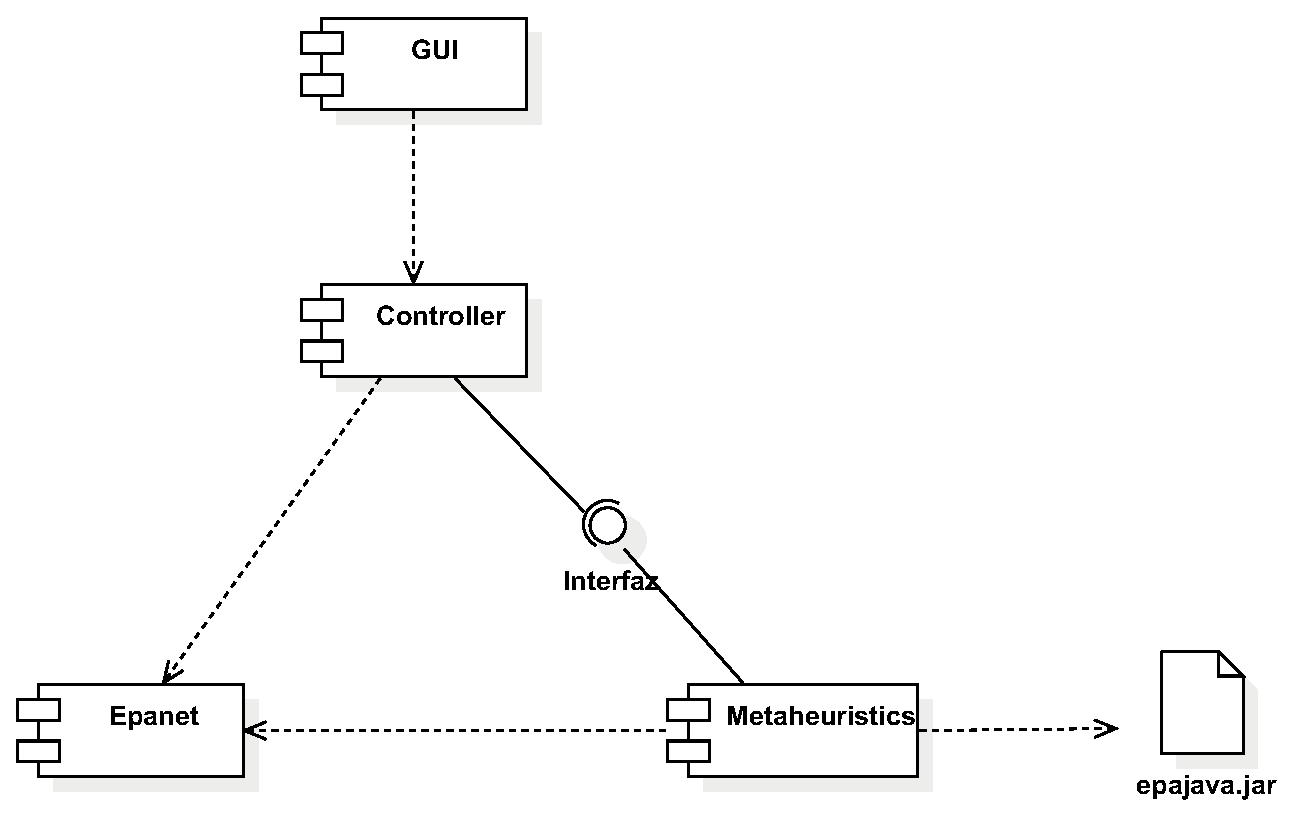
\includegraphics[width=\textwidth]{Capitulo3/assets/diagrama_de_componentes.eps}
    \caption{Diagrama de componentes.}
    \label{fig:diagrama_componentes}
\end{figure}

A continuaci�n, se describe cada uno de los componentes presentados en la Figura \ref{fig:diagrama_componentes}:

\begin{description}
    \item[\textit{GUI (Graphics User Interface)}]	Este componente este encargado de presentar todas las vistas. Entre las vistas se encuentra la ventana principal de la aplicaci�n, la ventana de configuraci�n de para un problema, la ventana de ejecuci�n de algoritmos y la ventana de resultados.
    \item[\textit{Controller}]	El controlador se encarga de manejar los eventos generados por la \textit{GUI}. Generalmente la relaci�n es uno a uno, es decir, por cada interfaz de usuario hay un controlador. Debido a que dentro de la interfaz de usuario est� formada por varios componentes, se da el caso en que cada uno de estos componentes puede tener su propio controlador. 
    \item[Epanet]	Este componente esta encargada de la lectura y la escritura de archivos inp. Este componente cuenta tambi�n con clases que representan una red cargada desde un inp. Estas clases permitir�n editar, durante la ejecuci�n del programa, algunas configuraciones de la red con el fin de crear un nuevo archivo de descripci�n de la red.
    \item[\textit{Metaheuristics}]	Este componente contiene los algoritmos metaheur�sticos, as� como los problemas y los operadores que pueden ser ocupados por los algoritmos.
    \item[epajava.jar]	Esta es una librer�a para la simulaci�n de las redes de agua potable. Esta librer�a permite realizar llamadas nativas a la librer�a de Epanet. Estas llamadas nativas se hacen a trav�s de la librer�a \textit{JNA (Java Native Access)}. Para ocupar la librer�a, esta requiere que se indique el archivo de descripci�n de la red (Archivo inp).
\end{description}

